\begin{frame}{Utilité des caches}
	\begin{columns}[c]
		\begin{column}{.5\textwidth}
			\begin{figure}[h!]
				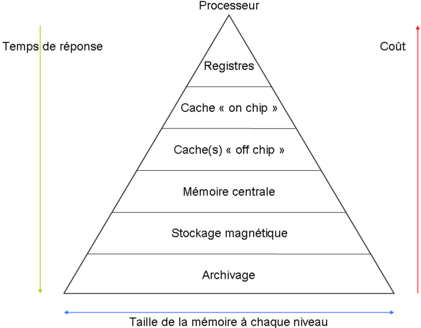
\includegraphics[scale=.45]{images/hierarchy.png}
			\end{figure}
		\end{column}
		\begin{column}{.5\textwidth}
			\begin{block}{Objectif}
				\begin{itemize}
					\item{Trouver un bon compromis entre vitesse et coût}
				\end{itemize}
			\end{block}
		\end{column}
	\end{columns}
	\begin{block}{\emph{Cache hit} et \emph{cache miss}}
		\begin{itemize}
			\item{Si le processeur trouve la donnée recherchée dans le cache : il fait un \emph{hit}}
			\item{Sinon, la donnée est rapatriée à partir de la mémoire de niveau supérieur : c'est un \emph{miss}}			
			\end{itemize}
	\end{block}
\end{frame}


\begin{frame}{Structure d'un cache}
	\begin{columns}[c]
		\begin{column}{.6\textwidth}
			On utilise plusieurs niveaux de caches
		\end{column}
		\begin{column}{.4\textwidth}
			\begin{figure}[h!]
				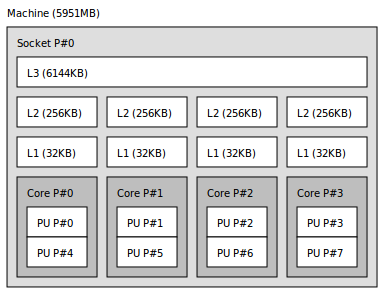
\includegraphics[scale=.3]{images/lstopo.png}
			\end{figure}
		\end{column}
	\end{columns}
	
	+ parler des lignes de caches et d'étiquettes...
\end{frame}	

\begin{frame}{Associativité}
	\begin{block}{Fonction de correspondance adresse mémoire / cache}
		\begin{itemize}
			\item{Direct associative}
			\item{Fully associative}
			\item{k-ways associative}
		\end{itemize}
	\end{block}
	\begin{figure}[h!]
		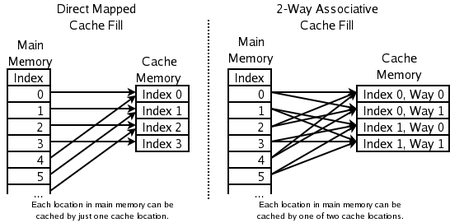
\includegraphics[scale=.33]{images/associative.png}
	\end{figure}
\end{frame}

\begin{frame}{Remplacement}
	\begin{block}{Comment ajouter une donnée dans set plein ?}
		Il existe différentes politiques de remplacement
		\begin{itemize}
			\item{FIFO (Supprimer la plus ancienne)}
			\item{LFU (Supprimer la moins utilisée)}
			\item{LRU (Supprimer la plus anciennement utilisée)}
		\end{itemize}
		Les données évincées sont déplacées vers la mémoire de niveau supérieur
	\end{block}
\end{frame}

\begin{frame}{Hiérarchie de caches et problèmes de cohérence}
\begin{block}{Comment gérer les données entre différents niveaux?}
		\begin{itemize}
			\item{Caches inclusifs/exclusifs}
		\end{itemize}
	\end{block}
	+ Parler de write-through / write-back
	\begin{block}{Comment gérer les données entre caches de même niveau?}
		Que faire lorsque deux caches doivent se partager une même donnée ?
	\end{block}
\end{frame}
